\section{Results}
\label{sec:results}

All results in this section are from the pre-registered EEHDA benchmark across 25 evaluation seeds. The benchmark is a controlled, fully reproducible measurement of prioritization quality; \S\ref{sec:external_validity} quantifies how the headline gap behaves under real EPSS/KEV attribute distributions.

\subsection{Precision@$K$: All Methods Across $K = 50, 100, 250$}

Table~\ref{tab:precision_k} reports mean P@$K$ and BCa 95\% CI for all nine methods at $K = 50, 100$, and $250$. The following observations emerge from the results.

\begin{table*}[!t]
 \caption{Precision@$K$ across all methods (25 evaluation seeds). BCa 95\% CI, 10,000 resamples. Frozen results from \texttt{primary\_results\_v1/\allowbreak primary\_results.csv} (225 rows: 25 seeds $\times$ 9 methods).}
 \label{tab:precision_k}
 \centering
 \begin{tabular}{llll}
 \toprule
 \textbf{Method} & \textbf{P@50 mean (95\% CI)} & \textbf{P@100 mean (95\% CI)} & \textbf{P@250 mean (95\% CI)} \\
 \midrule
 HygienePrio-full & 0.509 (0.480-0.542) & 0.458 (0.441-0.474) & 0.420 (0.408-0.432) \\
 HygienePrio-noFreshness & 0.490 (0.463-0.528) & 0.446 (0.426-0.463) & 0.411 (0.398-0.422) \\
 HygienePrio-noInteraction & 0.482 (0.454-0.515) & 0.445 (0.428-0.462) & 0.417 (0.405-0.430) \\
 HygienePrio-noAD & 0.424 (0.395-0.460) & 0.379 (0.362-0.398) & 0.370 (0.357-0.382) \\
 HygienePrio-noPatch & 0.312 (0.283-0.343) & 0.289 (0.270-0.309) & 0.284 (0.273-0.294) \\
 HRS-only & 0.288 (0.263-0.310) & 0.284 (0.265-0.304) & 0.282 (0.271-0.291) \\
 EPSS-only & 0.202 (0.174-0.236) & 0.199 (0.185-0.218) & 0.215 (0.205-0.226) \\
 CVSS-only & 0.056 (0.044-0.069) & 0.056 (0.046-0.065) & 0.057 (0.052-0.061) \\
 Random & 0.048 (0.039-0.056) & 0.062 (0.054-0.071) & 0.061 (0.055-0.067) \\
 \bottomrule
 \end{tabular}
\end{table*}

\begin{table*}[!t]
 \caption{NDCG@$K$ across all methods (25 evaluation seeds). BCa 95\% CI, 10,000 resamples. Binary relevance: rel$(h,c) \in \{0,1\}$ per ground truth definition (\S3).}
 \label{tab:ndcg_k}
 \centering
 \begin{tabular}{llll}
 \toprule
 \textbf{Method} & \textbf{NDCG@50 mean (95\% CI)} & \textbf{NDCG@100 mean (95\% CI)} & \textbf{NDCG@250 mean (95\% CI)} \\
 \midrule
 HygienePrio-full & 0.556 (0.521-0.591) & 0.499 (0.478-0.519) & 0.501 (0.485-0.515) \\
 HygienePrio-noFreshness & 0.536 (0.502-0.572) & 0.484 (0.462-0.507) & 0.488 (0.473-0.502) \\
 HygienePrio-noInteraction & 0.524 (0.488-0.558) & 0.479 (0.457-0.500) & 0.491 (0.475-0.506) \\
 HygienePrio-noAD & 0.464 (0.426-0.502) & 0.414 (0.390-0.439) & 0.435 (0.419-0.450) \\
 HygienePrio-noPatch & 0.334 (0.302-0.367) & 0.308 (0.287-0.330) & 0.328 (0.315-0.342) \\
 HRS-only & 0.297 (0.266-0.329) & 0.291 (0.269-0.313) & 0.319 (0.307-0.331) \\
 EPSS-only & 0.202 (0.171-0.234) & 0.199 (0.181-0.220) & 0.237 (0.225-0.250) \\
 CVSS-only & 0.063 (0.047-0.082) & 0.060 (0.048-0.073) & 0.066 (0.059-0.073) \\
 Random & 0.051 (0.040-0.063) & 0.061 (0.052-0.070) & 0.068 (0.062-0.074) \\
 \bottomrule
 \end{tabular}
\end{table*}

NDCG@$K$ results (Table~\ref{tab:ndcg_k}) are consistent with P@$K$: HygienePrio-full leads all methods at all $K$ values with non-overlapping CIs against EPSS-only (NDCG@50: 0.556 vs.\ 0.202; NDCG@100: 0.499 vs.\ 0.199). The NDCG pattern mirrors P@$K$ because the ground truth uses binary relevance (rel $\in \{0,1\}$); graded relevance would require per-pair exploitation probability estimates, which the benchmark does not define.

\begin{figure}[t]
 \centering
 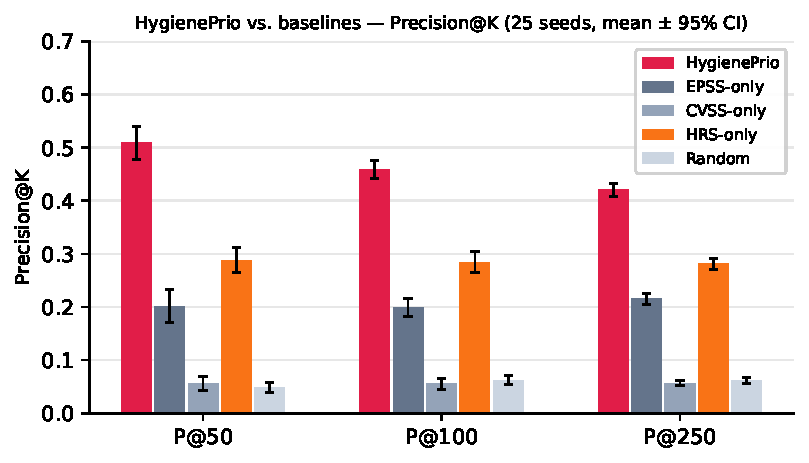
\includegraphics[width=\columnwidth]{figures/fig1_precision_at_k}
 \caption{Mean Precision@$K$ ($K \in \{50,100,250\}$) for all methods across 25 evaluation seeds (mean $\pm$ 95\% BCa CI). HygienePrio consistently outperforms all baselines at every $K$.\\[2pt]\textit{Alt text:} A grouped chart with the vertical axis showing mean Precision@$K$ and grouped along $K = 50, 100, 250$, comparing the nine methods. Each point carries a 95\% confidence-interval error bar. The HygienePrio variants sit highest, while EPSS-only, CVSS-only, and Random sit progressively lower at every value of $K$.}
 \label{fig:precision_k}
\end{figure}

\textbf{HygienePrio-full vs.\ EPSS-only.} HygienePrio-full achieves a mean P@50 of 0.509 compared with EPSS-only's 0.202, an approximately 31 pp improvement, with non-overlapping BCa CIs (0.480-0.542 vs.\ 0.174-0.236). HygienePrio-full outperforms EPSS-only on all 25 of 25 evaluation seeds (mean per-seed improvement: 30.7 pp). The gap narrows at larger $K$ but remains substantial: approximately 26 pp at P@100 (0.458 vs.\ 0.199) and 21 pp at P@250 (0.420 vs.\ 0.215). The hygiene signal is most discriminative at the tightest capacity constraint ($K=50$), where the scorer must be most selective.

\textbf{H1 assessment.} The observed improvement of approximately 31 pp at P@50 substantially exceeds the pre-registered H1 threshold of $\geq$5 pp, supporting H1. The BCa CIs for HygienePrio-full and EPSS-only do not overlap at any $K$ value, providing strong support for the hypothesis that hygiene signals add prioritization value beyond EPSS alone. \S\ref{sec:external_validity} quantifies how this benchmark gap behaves under real EPSS/KEV attribute distributions, where the aggregate margin is smaller but the host-side discrimination at major-CVE disclosure moments persists (\S9.2).

\textbf{EPSS-only vs.\ CVSS-only.} Consistent with prior literature~\cite{jacobs2021epss,jacobs2020improving} and the VulnPrio study, EPSS substantially outperforms CVSS-only at all $K$ values (0.202 vs.\ 0.056 at P@50), reinforcing that exploit likelihood is a better prioritization signal than intrinsic severity. This replication of the VulnPrio study finding on a different metric (P@$K$ vs.\ EHD) provides internal consistency.

\textbf{HRS-only vs.\ EPSS-only.} HRS-only (host hygiene without CVE signal) achieves 0.288 at P@50 versus EPSS-only's 0.202, approximately 9 pp higher, with non-overlapping CIs. However, HygienePrio-full (0.509) substantially outperforms HRS-only (0.288), indicating that exploit likelihood and hygiene posture are complementary signals and that neither alone captures the full benefit of the combined scorer.

\begin{figure}[t]
 \centering
 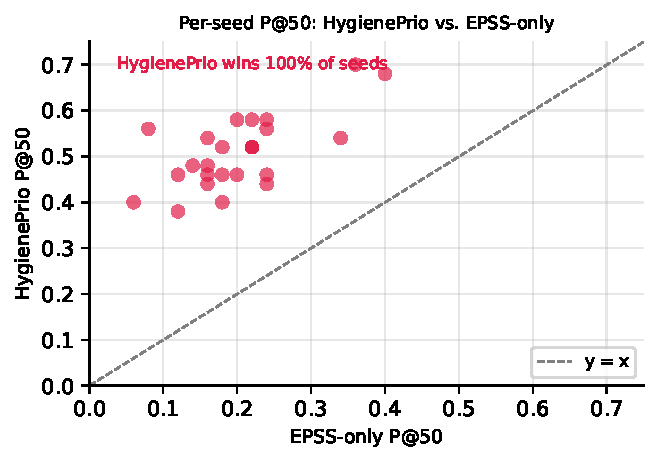
\includegraphics[width=\columnwidth]{figures/fig3_seed_scatter}
 \caption{Per-seed P@50 for HygienePrio-full vs.\ EPSS-only (25 seeds). Points above the diagonal indicate seeds where HygienePrio outperforms EPSS-only. HygienePrio wins on all 25 of 25 evaluation seeds.\\[2pt]\textit{Alt text:} A scatter plot with one point per evaluation seed, where the horizontal axis is EPSS-only P@50 and the vertical axis is HygienePrio-full P@50, with a diagonal line marking equal performance. All 25 points fall above the diagonal, showing HygienePrio-full scores higher than EPSS-only on every seed.}
 \label{fig:seed_scatter}
\end{figure}

\subsection{Ablation: Hygiene Dimension Contributions}

Table~\ref{tab:ablation} presents the ablation results, comparing HygienePrio-full with three leave-one-dimension-out variants. Results are for P@50.

\begin{table}[!t]
 \caption{Ablation, P@50 impact of removing each hygiene dimension. Ablation uses fixed ground-truth labels (HRS from calibrated weights); only scorer's HRS input changes.}
 \label{tab:ablation}
 \centering
 \small
 \setlength{\tabcolsep}{3pt}
 \begin{tabular}{>{\raggedright}p{2.5cm}
 >{\raggedright}p{2.0cm}
 >{\raggedright}p{1.2cm}
 >{\raggedright\arraybackslash}p{1.1cm}}
 \toprule
 \textbf{Condition} & \textbf{P@50 (95\%~CI)} & \textbf{Drop} & \textbf{CI overlap?} \\
 \midrule
 Full model & 0.509 (0.480-0.542) &, &, \\
 noPatch ($w_1{=}0$)& 0.312 (0.283-0.343) & $-$20 pp & No \\
 noAD ($w_2{=}0$) & 0.424 (0.395-0.460) & $-$9 pp & No \\
 noFreshness ($w_3{=}0$) & 0.490 (0.463-0.528) & $-$2 pp & Yes \\
 \bottomrule
 \end{tabular}
\end{table}

\textbf{H2 assessment.} The patch posture dimension shows the largest marginal contribution: removing it (HygienePrio-noPatch) drops P@50 by approximately 20 pp (0.509 $\to$ 0.312), with non-overlapping BCa CIs, strongly supporting H2. The AD exposure dimension shows a substantial secondary contribution ($\sim$9 pp drop, non-overlapping CIs). Telemetry freshness shows the smallest contribution ($\sim$2 pp drop, overlapping CIs, indicating marginal discriminative power). This result is consistent with HygieneBench Task T5's finding that patch-vulnerability hygiene carries the most discriminative signal among hygiene dimensions.

The dimension ordering (patch posture $>$ AD exposure $\gg$ freshness) suggests that operations teams seeking to deploy a simplified HygienePrio variant should prioritize patch posture instrumentation first, AD group exposure tracking second, and telemetry freshness monitoring last.

\begin{figure}[t]
 \centering
 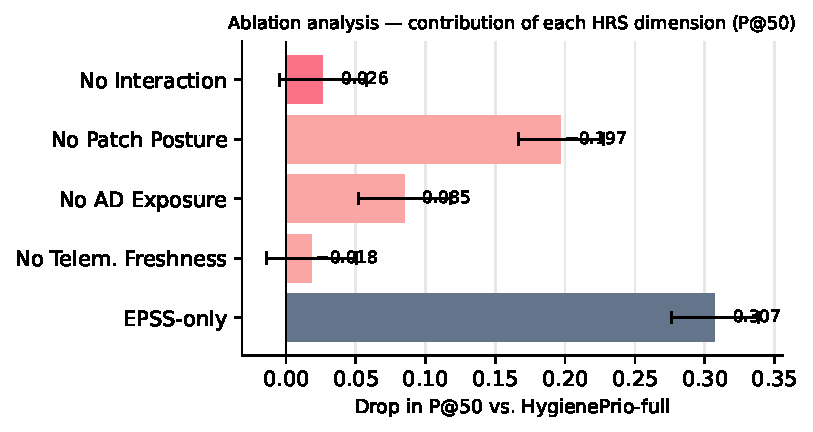
\includegraphics[width=\columnwidth]{figures/fig2_ablation}
 \caption{Ablation analysis: drop in P@50 from HygienePrio-full when each dimension or component is removed (25 seeds, mean $\pm$ 95\% BCa CI). Patch posture is the dominant contributor ($\approx$20\,pp); AD exposure contributes $\approx$9\,pp; telemetry freshness and the interaction term contribute marginally (approximately 3\,pp).\\[2pt]\textit{Alt text:} A bar chart where each bar shows the drop in P@50 (in percentage points) caused by removing one model component, with 95\% confidence-interval error bars. The patch-posture bar is the tallest at about 20 points, the AD-exposure bar about 9 points, and the telemetry-freshness and interaction-term bars are smallest at about 3 points.}
 \label{fig:ablation}
\end{figure}

\subsection{Interaction Term Analysis}

Comparing HygienePrio-full with HygienePrio-noInteraction reveals approximately 3 pp improvement at P@50 from including the interaction term ($\mathrm{EPSS} \times \mathrm{HRS}$) (0.509 vs.\ 0.482). The BCa CIs overlap substantially (0.480-0.542 vs.\ 0.454-0.515), so the interaction term's contribution is marginal. At P@100 and P@250 the difference narrows further ($\sim$1 pp). The interaction term's modest contribution reflects the EPSS distribution: high-EPSS and high-HRS pair conjunctions are relatively rare ($\sim$10-12\% of applicable pairs per seed), limiting opportunities for the interaction term to add discriminative value.

Per the pre-registration stop rule, if HygienePrio-noInteraction achieves P@$K$ within 1 pp of HygienePrio-full for all $K$, the interaction term would be declared uninformative. At P@50 the difference exceeds 1 pp (3 pp), so the interaction term is retained in the reported full model. The overlapping CIs mean this finding is equivocal: the interaction term likely does not materially change prioritization decisions under the distributions evaluated here.

\subsection{Oracle-Gap Analysis}

\begin{table}[!t]
 \caption{Oracle-gap (\%) at $K = 50$ by method (BCa 95\% CI)}
 \label{tab:oracle_gap}
 \centering
 \small
 \setlength{\tabcolsep}{4pt}
 \begin{tabular}{>{\raggedright}p{2.6cm}
 >{\raggedright}p{2.3cm}
 >{\raggedright\arraybackslash}p{2.4cm}}
 \toprule
 \textbf{Method} & \textbf{Oracle-gap (95\%~CI)} & \textbf{P@50 captured} \\
 \midrule
 HygienePrio-full & 49.1\% (45.6-51.8\%) & $\sim$51\% of oracle \\
 EPSS-only & 79.8\% (76.3-82.6\%) & $\sim$20\% of oracle \\
 CVSS-only & 94.4\% (93.0-95.5\%) & $\sim$6\% of oracle \\
 Random & 95.2\% (94.2-96.0\%) & $\sim$5\% of oracle \\
 \bottomrule
 \end{tabular}
\end{table}

The oracle-gap analysis indicates that even HygienePrio-full captures approximately 51\% of theoretically achievable precision at $K=50$, leaving substantial room for improvement. The gap between HygienePrio-full and the oracle (49.1\%) reflects both the inherent difficulty of the ranking problem and the residual uncertainty in hygiene signals: among hygiene-poor hosts with similar HRS values, the scorer cannot further discriminate which specific CVE-host pair is the highest-priority target. At $K=50$, with approximately 175-250 true positives per seed (mean $\approx$217), the maximum achievable P@50 is 1.0 (oracle), and HygienePrio-full achieves 0.509. The 49.1\% oracle gap is substantially smaller than EPSS-only's 79.8\% gap, confirming that hygiene signals materially reduce the distance from optimal prioritization.

\subsection{Summary of Main Findings}

The results support the following findings on the benchmark:

\begin{enumerate}
 \item \textbf{HygienePrio-full improves over EPSS-only by approximately 31 pp} at P@50 (0.509 vs.\ 0.202), with non-overlapping BCa CIs, substantially exceeding the pre-registered H1 threshold ($\geq$5 pp). Improvement is 26 pp at P@100 and 21 pp at P@250. \S9.2 and \S\ref{sec:external_validity} characterize how much of this margin is attributable to the benchmark's labelling rule and CVE attribute distribution.
 \item \textbf{Patch posture is the dominant hygiene dimension}, contributing approximately 20 pp to P@50 in the leave-one-out ablation (0.509 $\to$ 0.312 without patch posture), with non-overlapping CIs, strongly supporting H2.
 \item \textbf{AD exposure is a substantial secondary contributor}, reducing P@50 by $\sim$9 pp when removed (0.509 $\to$ 0.424), with non-overlapping CIs.
 \item \textbf{The interaction term and telemetry freshness are marginal}: both show overlapping CIs with the full model, with contributions of $\sim$3 pp and $\sim$2 pp respectively. The pre-registration stop rule is not triggered at P@50 for the interaction term (3 pp $>$ 1 pp threshold), so both are retained in the full model.
 \item \textbf{HRS-only outperforms EPSS-only} by $\sim$9 pp (0.288 vs.\ 0.202), but the combination (HygienePrio-full, 0.509) substantially outperforms either signal alone, confirming that exploit likelihood and hygiene posture are complementary.
 \item \textbf{Oracle gap remains substantial}: HygienePrio-full captures $\sim$51\% of theoretically achievable P@50, versus $\sim$20\% for EPSS-only, indicating both that hygiene signals provide meaningful benefit and that significant room for improvement remains.
\end{enumerate}
